\documentclass[article]{beamer}
\usetheme{Warsaw}
\setbeamertemplate{footline}[frame number]

\usefonttheme[]{serif}
\usepackage{amsmath, latexsym, color, graphicx, amssymb, bm, here}
\usepackage{epsf, epsfig, pifont,tikz,subfigure}
\usepackage{graphics, calrsfs}
\usepackage{times}
\usepackage{fancybox,calc}
\usepackage{palatino,mathpazo}
\usepackage{amsfonts}
\usepackage{sidecap}
\usepackage{listings}
\usepackage{hyperref}

\title{Graph Theory: Introduction}
\author{David Jacobo \\ \href{mailto:jguillen@cimat.mx}{jguillen@cimat.mx}}
\date{\scriptsize{\today}}

\AtBeginSection[]
{
  \begin{frame}{Outline}
    \tableofcontents[currentsection]
  \end{frame}
}

\begin{document}

%%%%%%%%%%%%%%%%%%%%%%%%%%%%%%
\maketitle
			
%%%%%%%%%%%%%%%%%%%%%%%%%%%%%%
\begin{frame}
\frametitle{Definition}
\begin{center}
\huge
	G = (V, E)
	
\vspace{8mm}	
	
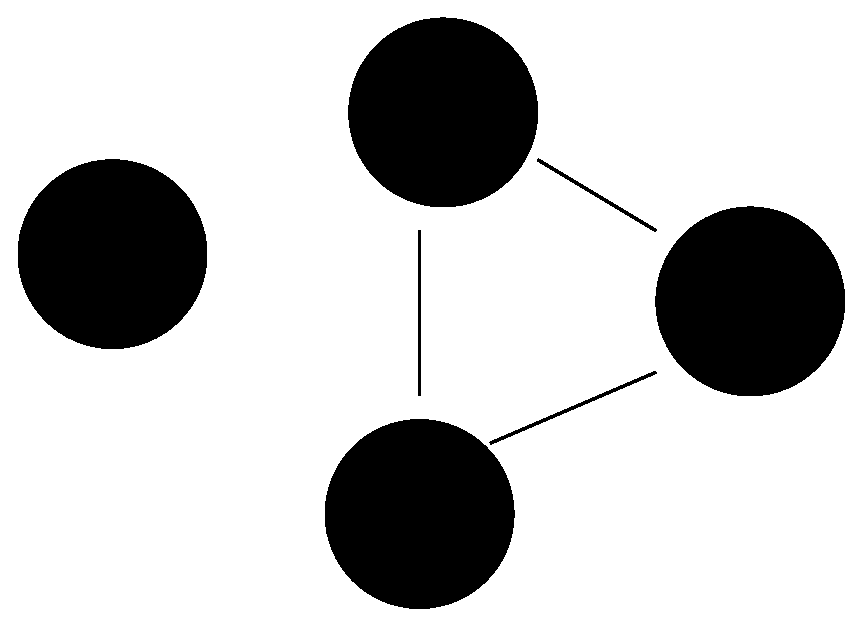
\includegraphics[scale=0.3]{./figures/graph.eps}
\end{center}
\end{frame}

%%%%%%%%%%%%%%%%%%%%%%%%%%%%%%

\section{Motivation}

\subsection{Seven Bridges of K\"onigsberg}
\begin{frame}
	\frametitle{Seven Bridges of K\"oninsberg}
	\begin{center}
	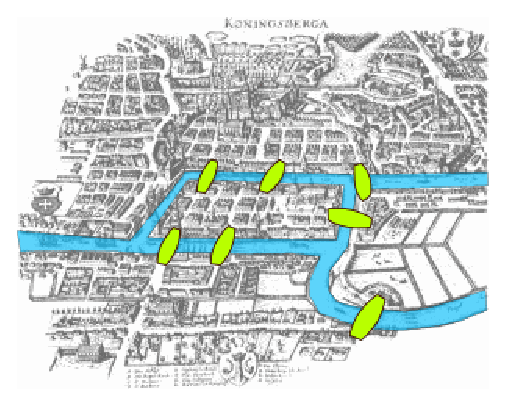
\includegraphics[scale=0.8]{./figures/kon.eps}
	\end{center}
	
	\begin{flushright} 
	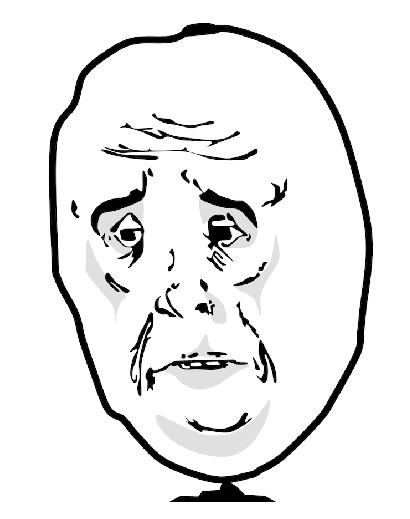
\includegraphics[scale=0.1]{./figures/okay.eps} "Okay" - Leonhard Euler \tiny (not really)
	\end{flushright}
	
\end{frame}

\subsection{Six degrees of separation theory}
\begin{frame}
	\frametitle{Six degrees of separation theory}
	"Six degrees of separation is the theory that everyone and everything is six or fewer steps away, by way of introduction, from any other person in the world ... It was originally set out by Frigyes Karinthy in 1929..." - Wikipedia
	
	\begin{center}
			\includegraphics[scale=0.3]{./figures/facebook.eps}
	\end{center}
\end{frame}

\subsection{More problems}
\begin{frame}
	\frametitle{Daily applications}
	\begin{columns}
		\column{.3\textwidth}
		Traffic
		\begin{center}
			\includegraphics[scale=0.2]{./figures/jam.eps}
		\end{center}
		\column{.3\textwidth}
		Traveling
		\begin{center}
			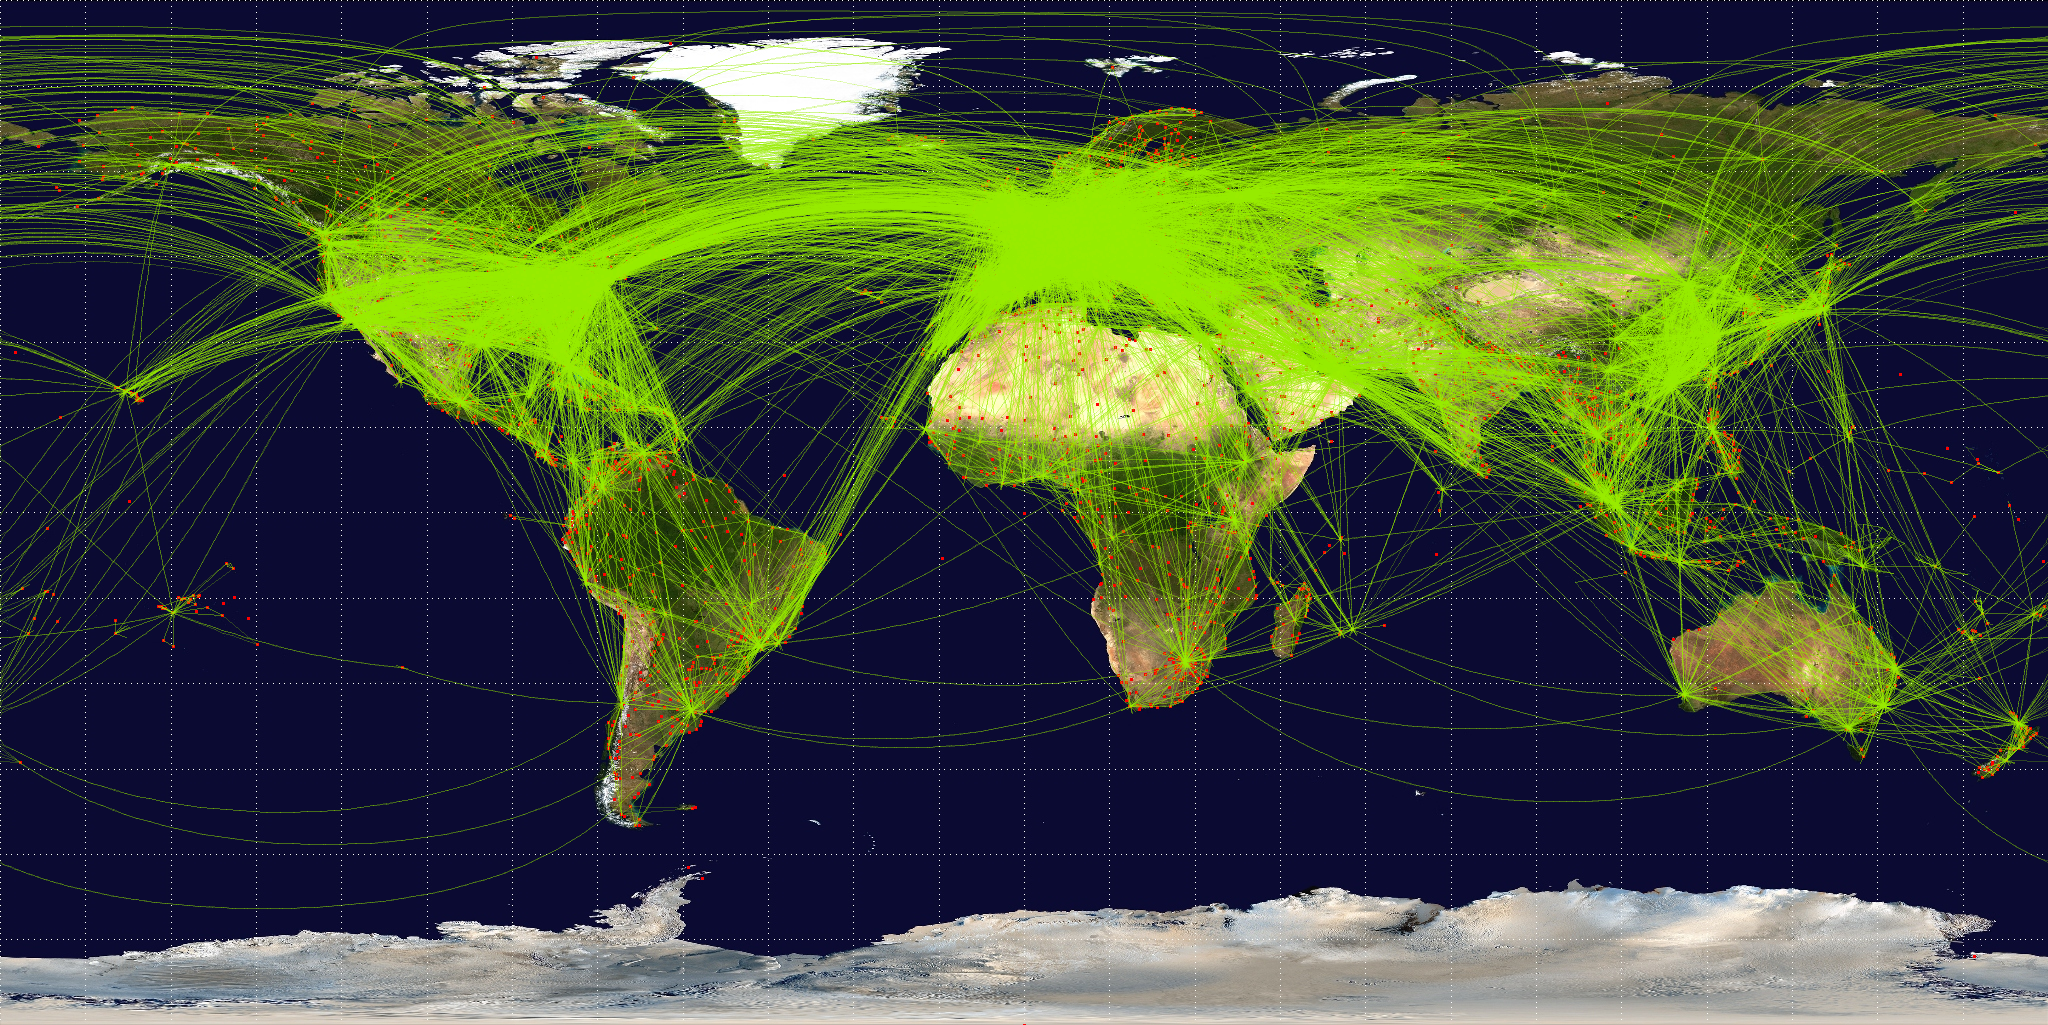
\includegraphics[scale=0.05]{./figures/airlines.png}
		\end{center}
		\column{.3\textwidth}
		Ranking
		\begin{center}
			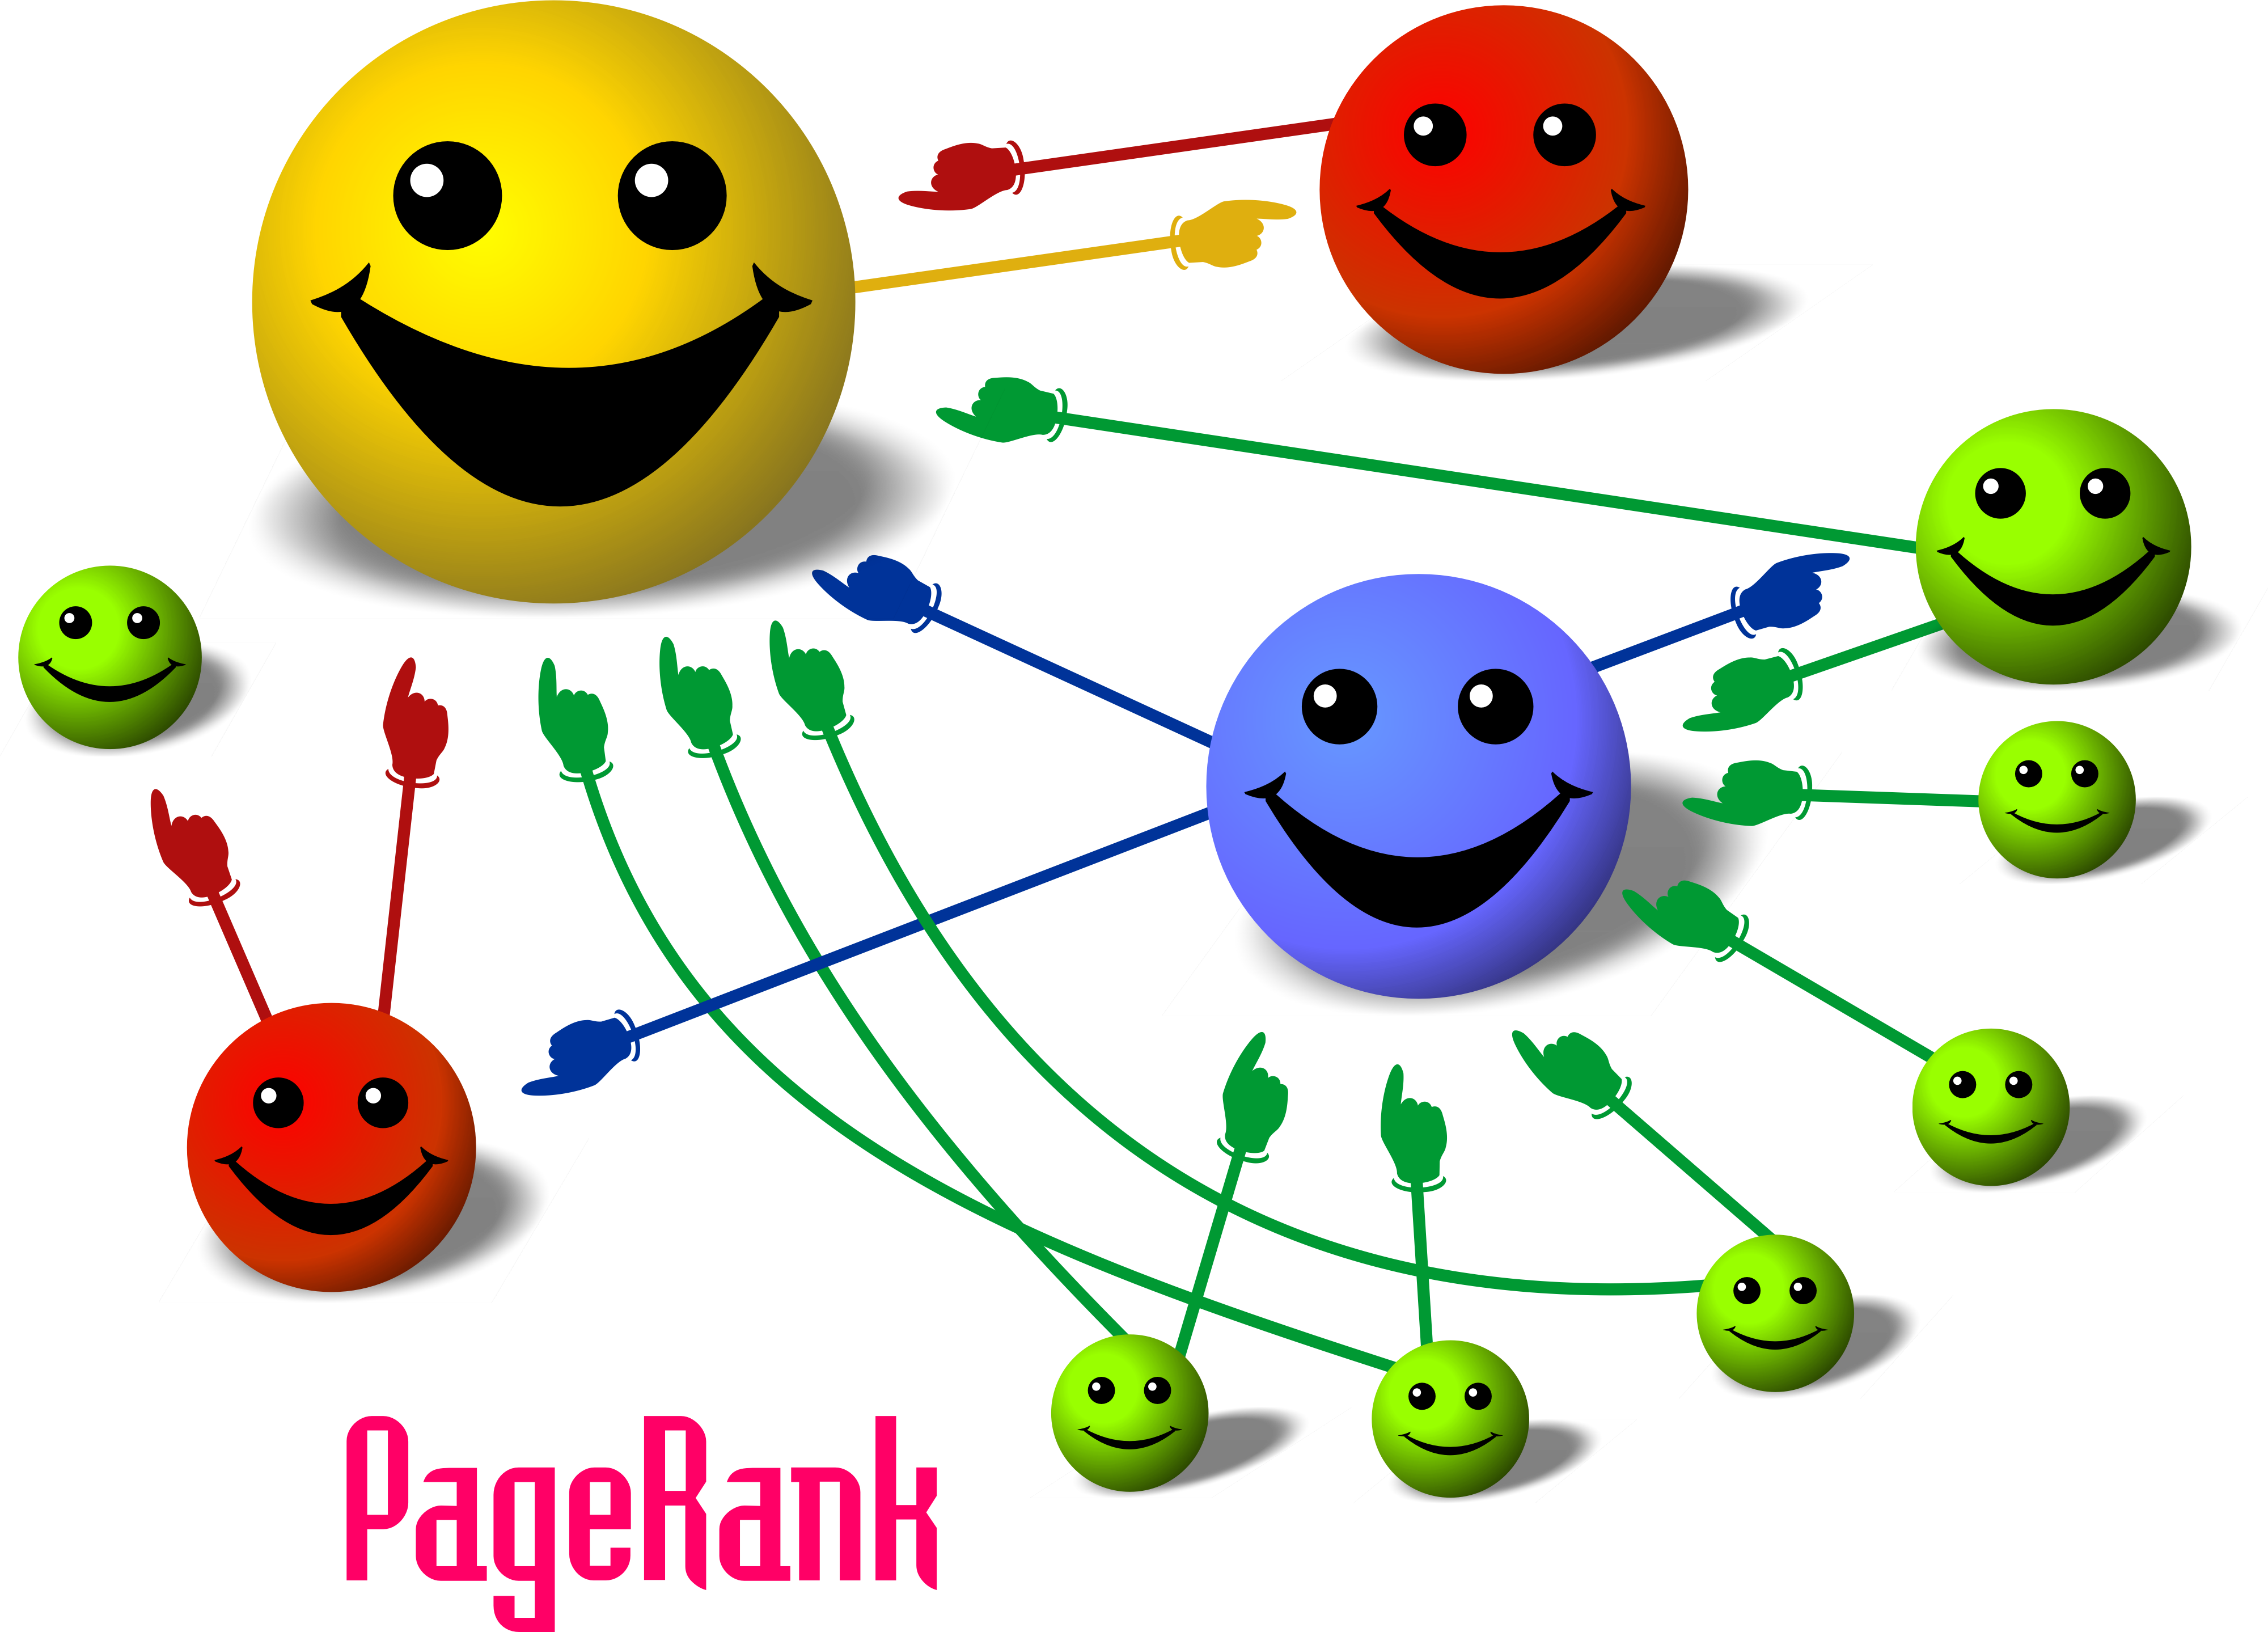
\includegraphics[scale=0.022]{./figures/pagerank.png}
		\end{center}
	\end{columns}
\end{frame}

\section{Graph theory basics}

\subsection{Terminology}
\begin{frame}
	\frametitle{Directed vs Undirected}
	\begin{columns}
		\column{.5\textwidth}
			\begin{center}
		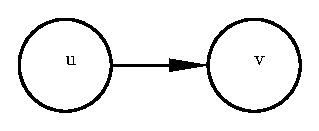
\includegraphics[scale=0.8]{./figures/directed.eps}
		\end{center}
		\column{.5\textwidth}
			\begin{center}
			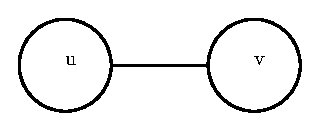
\includegraphics[scale=0.8]{./figures/undirected.eps}
			\end{center}
	\end{columns}
	
	\vspace{14mm}
	
	\begin{flushright} 
	For a directed graph, u $\rightarrow$ v doesn't imply v $\rightarrow$ u.
	\end{flushright}
\end{frame}

\begin{frame}
	\frametitle{Paths and cycles}
	\begin{center}
			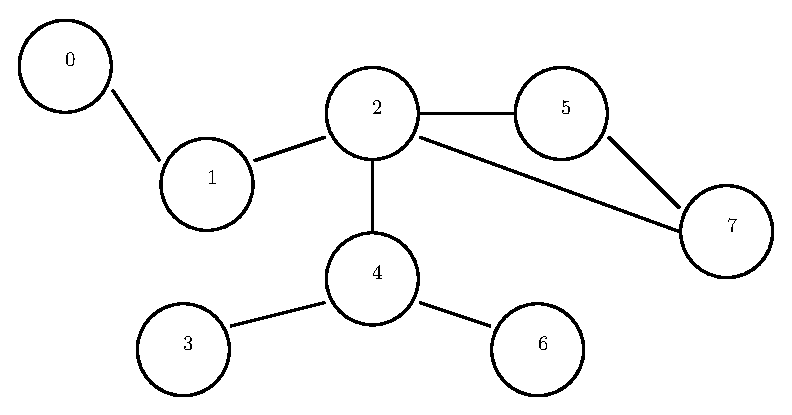
\includegraphics[scale=0.6]{./figures/path_cycle.eps}
	\end{center}
	
	\vspace{8mm}
	
	A path is a succession of distinct vertices which are connected. A cycle is also a path, in which the first and the last vertex are the same. 
\end{frame}

\begin{frame}
	\frametitle{Dense vs Sparse}
	\begin{columns}
		\column{.5\textwidth}
			\begin{center}
		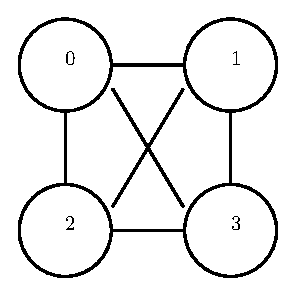
\includegraphics[scale=0.8]{./figures/dense.eps}
		\end{center}
		\column{.5\textwidth}
			\begin{center}
			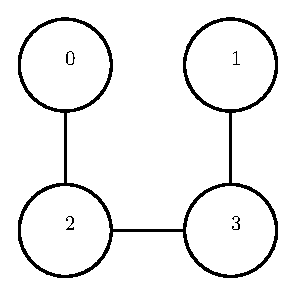
\includegraphics[scale=0.8]{./figures/sparse.eps}
			\end{center}
	\end{columns}
	
	\vspace{8mm}	
	
	\begin{flushright} 
	Leftmost figure is known as a \textbf{clique} and rightmost is a \textbf{tree}
	\end{flushright}
\end{frame}

\subsection{Graph representation}
\begin{frame}
	\frametitle{Adjacency Matrix}
	Having a \textbf{VxV matrix}, the space complexity for this is \textbf{O($V^2$)}. Preferred for dense graphs or for using with algorithms which constantly require to check if a particular edge exists.
	\begin{center}
			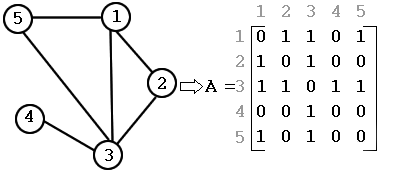
\includegraphics[scale=0.6]{./figures/AdjacencyMatrix.png}
	\end{center}
\end{frame}

\begin{frame}
	\frametitle{Adjacency List}
	List which contains the direct neighbours per each of the vertices, the memory space usage is \textbf{O(V + E)}. Preferred when our graph is sparse or the algorithm need to list the outgoing edges efficiently. 
	\begin{center}
			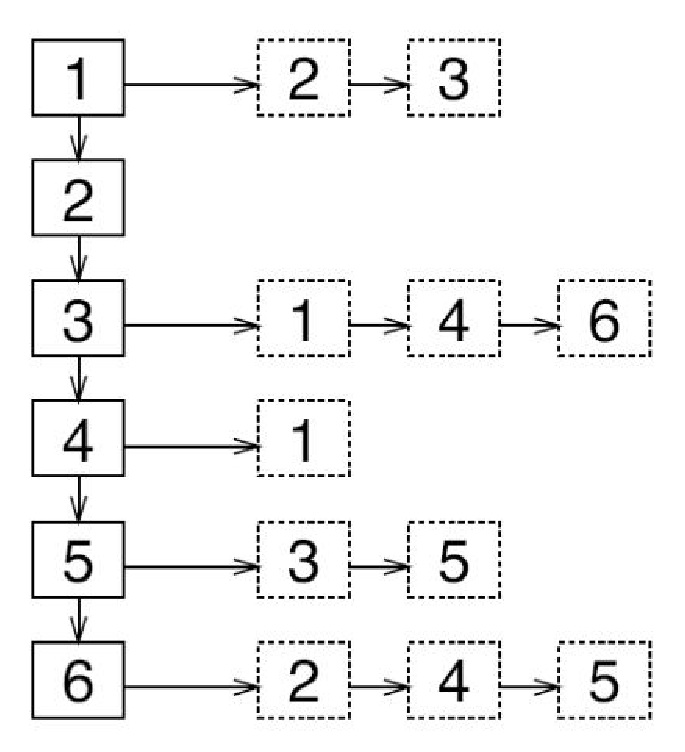
\includegraphics[scale=0.4]{./figures/adjacency_list.eps}
	\end{center}
\end{frame}

\section{Graph traversal}

\subsection{Deep First Search (DFS)}
\begin{frame}[fragile]
	\frametitle{DFS Algorithm}
	\begin{columns}
		\column{.6\textwidth}
		{\tiny
		\begin{lstlisting}
		Pre-requisite
			1     for each node n in G:            
	2         n.parent = NIL	
		
		1  DFS(G,v):
	2      label v as discovered
	3      for all valid edges v -> w do
	4          if vertex w !discovered then
	5               w.parent = v
	6              recursively call DFS(G,w)
		\end{lstlisting}
		}
		\column{.4\textwidth}
			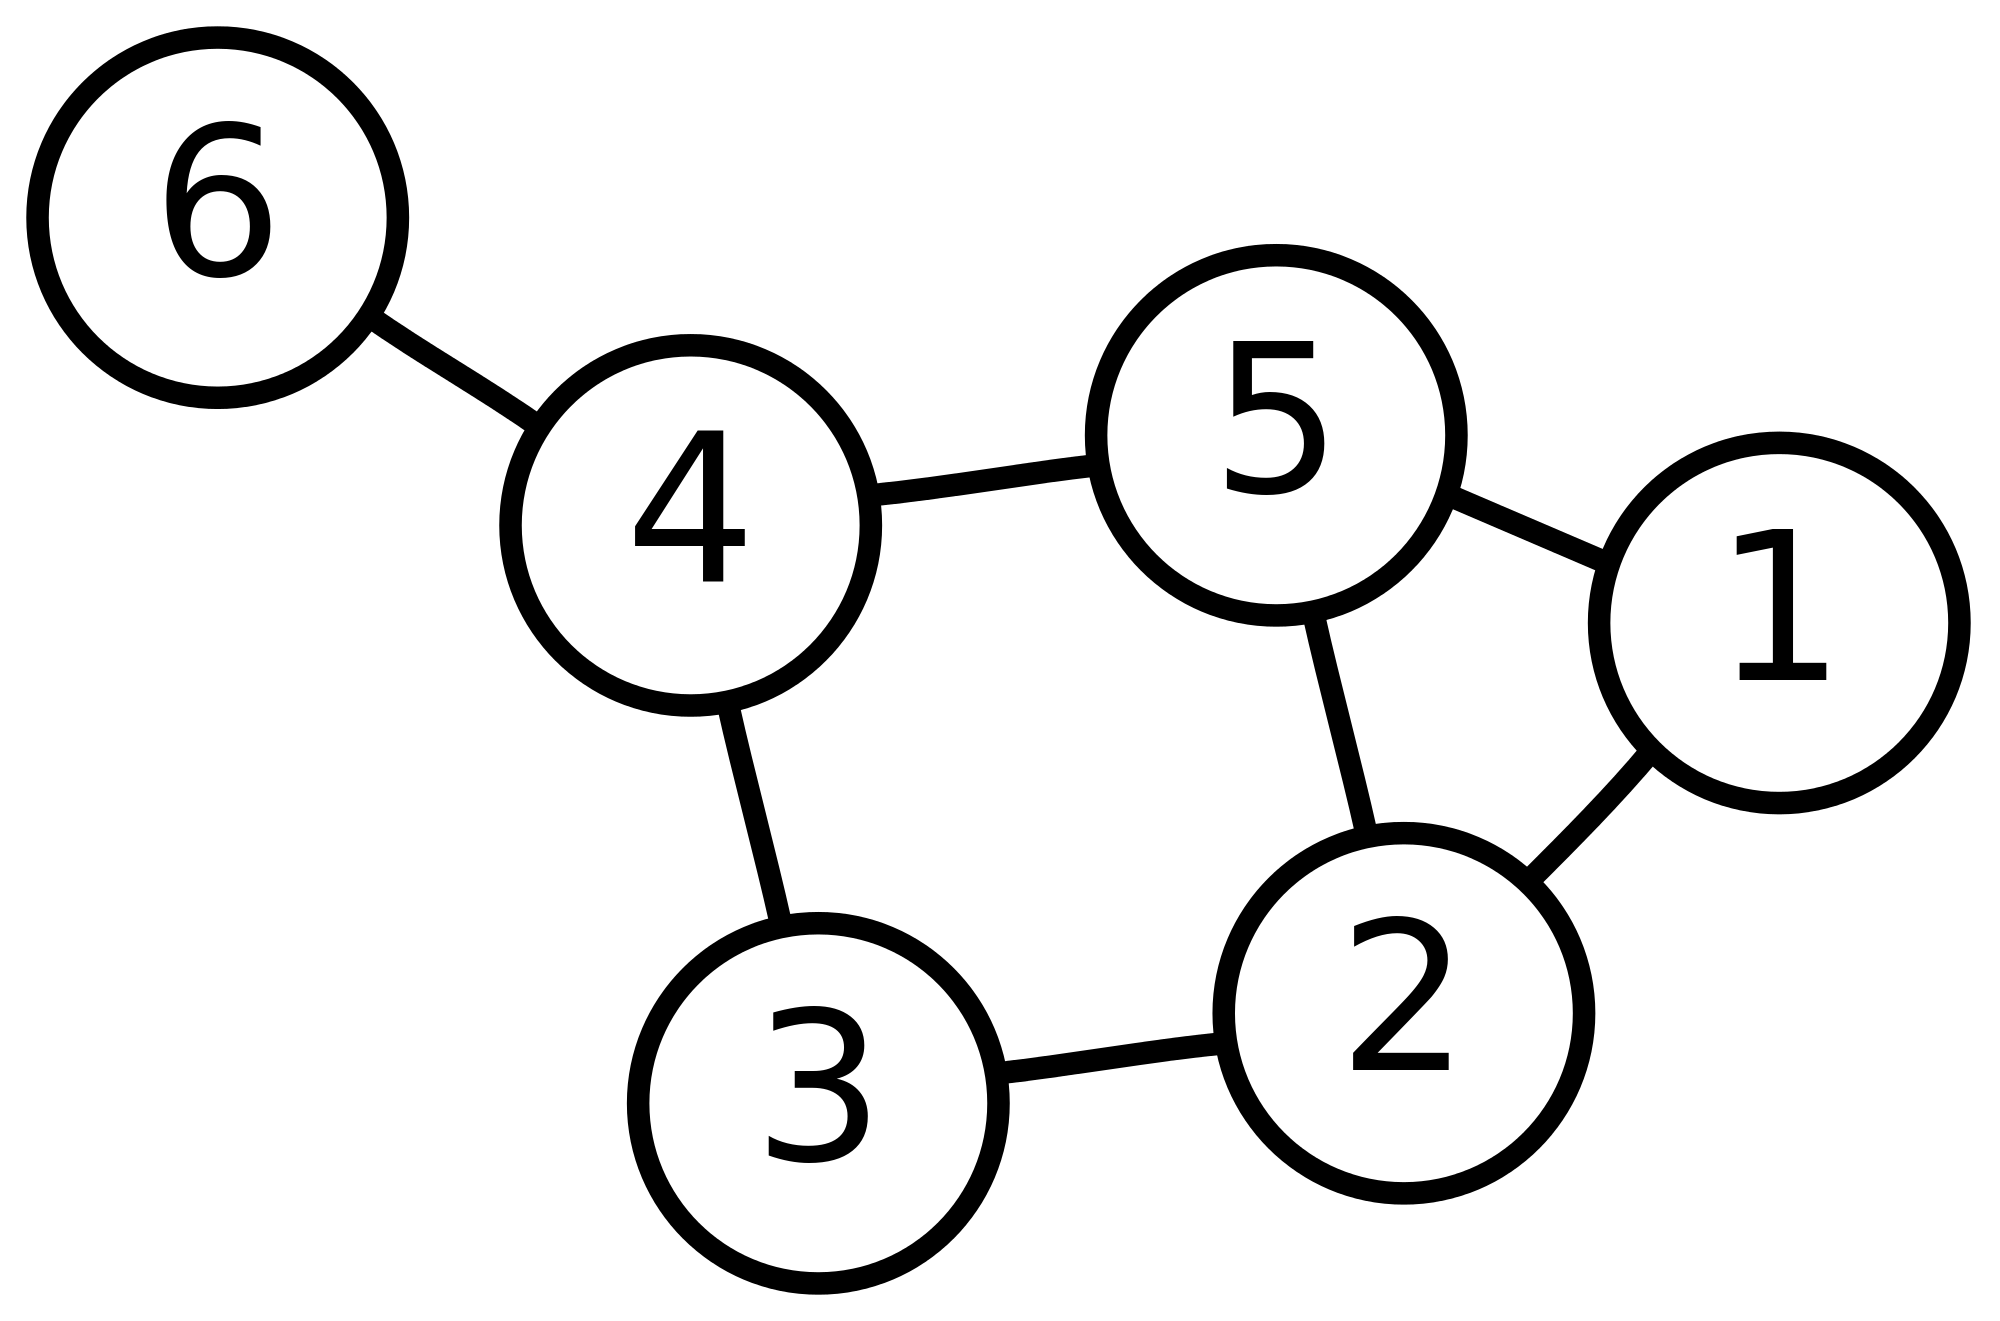
\includegraphics[scale=0.07]{./figures/graph_dfs_bfs.png}
	\end{columns}
	\begin{flushright} 
	Time complexity: \textbf{O(V+E)}
	\end{flushright}
\end{frame}

\subsection{Breadth First Search (BFS)}
\begin{frame}[fragile]
	\frametitle{BFS Algorithm}
	\begin{columns}
		\column{.6\textwidth}
		{\tiny
		\begin{lstlisting}
	 1 Breadth-First-Search(G, v):
	 2 
	 3     for each node n in G:            
	 4         n.distance = INFINITY        
	 5         n.parent = NIL
	 6 
	 7     create empty queue Q      
	 8 
	 9     v.distance = 0
	10     Q.enqueue(v)                      
	11 
	12     while Q is not empty:        
	13     
	14         u = Q.dequeue()
	15     
	16         for each node n that is adjacent to u:
	17             if n.distance == INFINITY:
	18                 n.distance = u.distance + 1
	19                 n.parent = u
	20                 Q.enqueue(n)
		\end{lstlisting}
		}
	\column{.4\textwidth}
			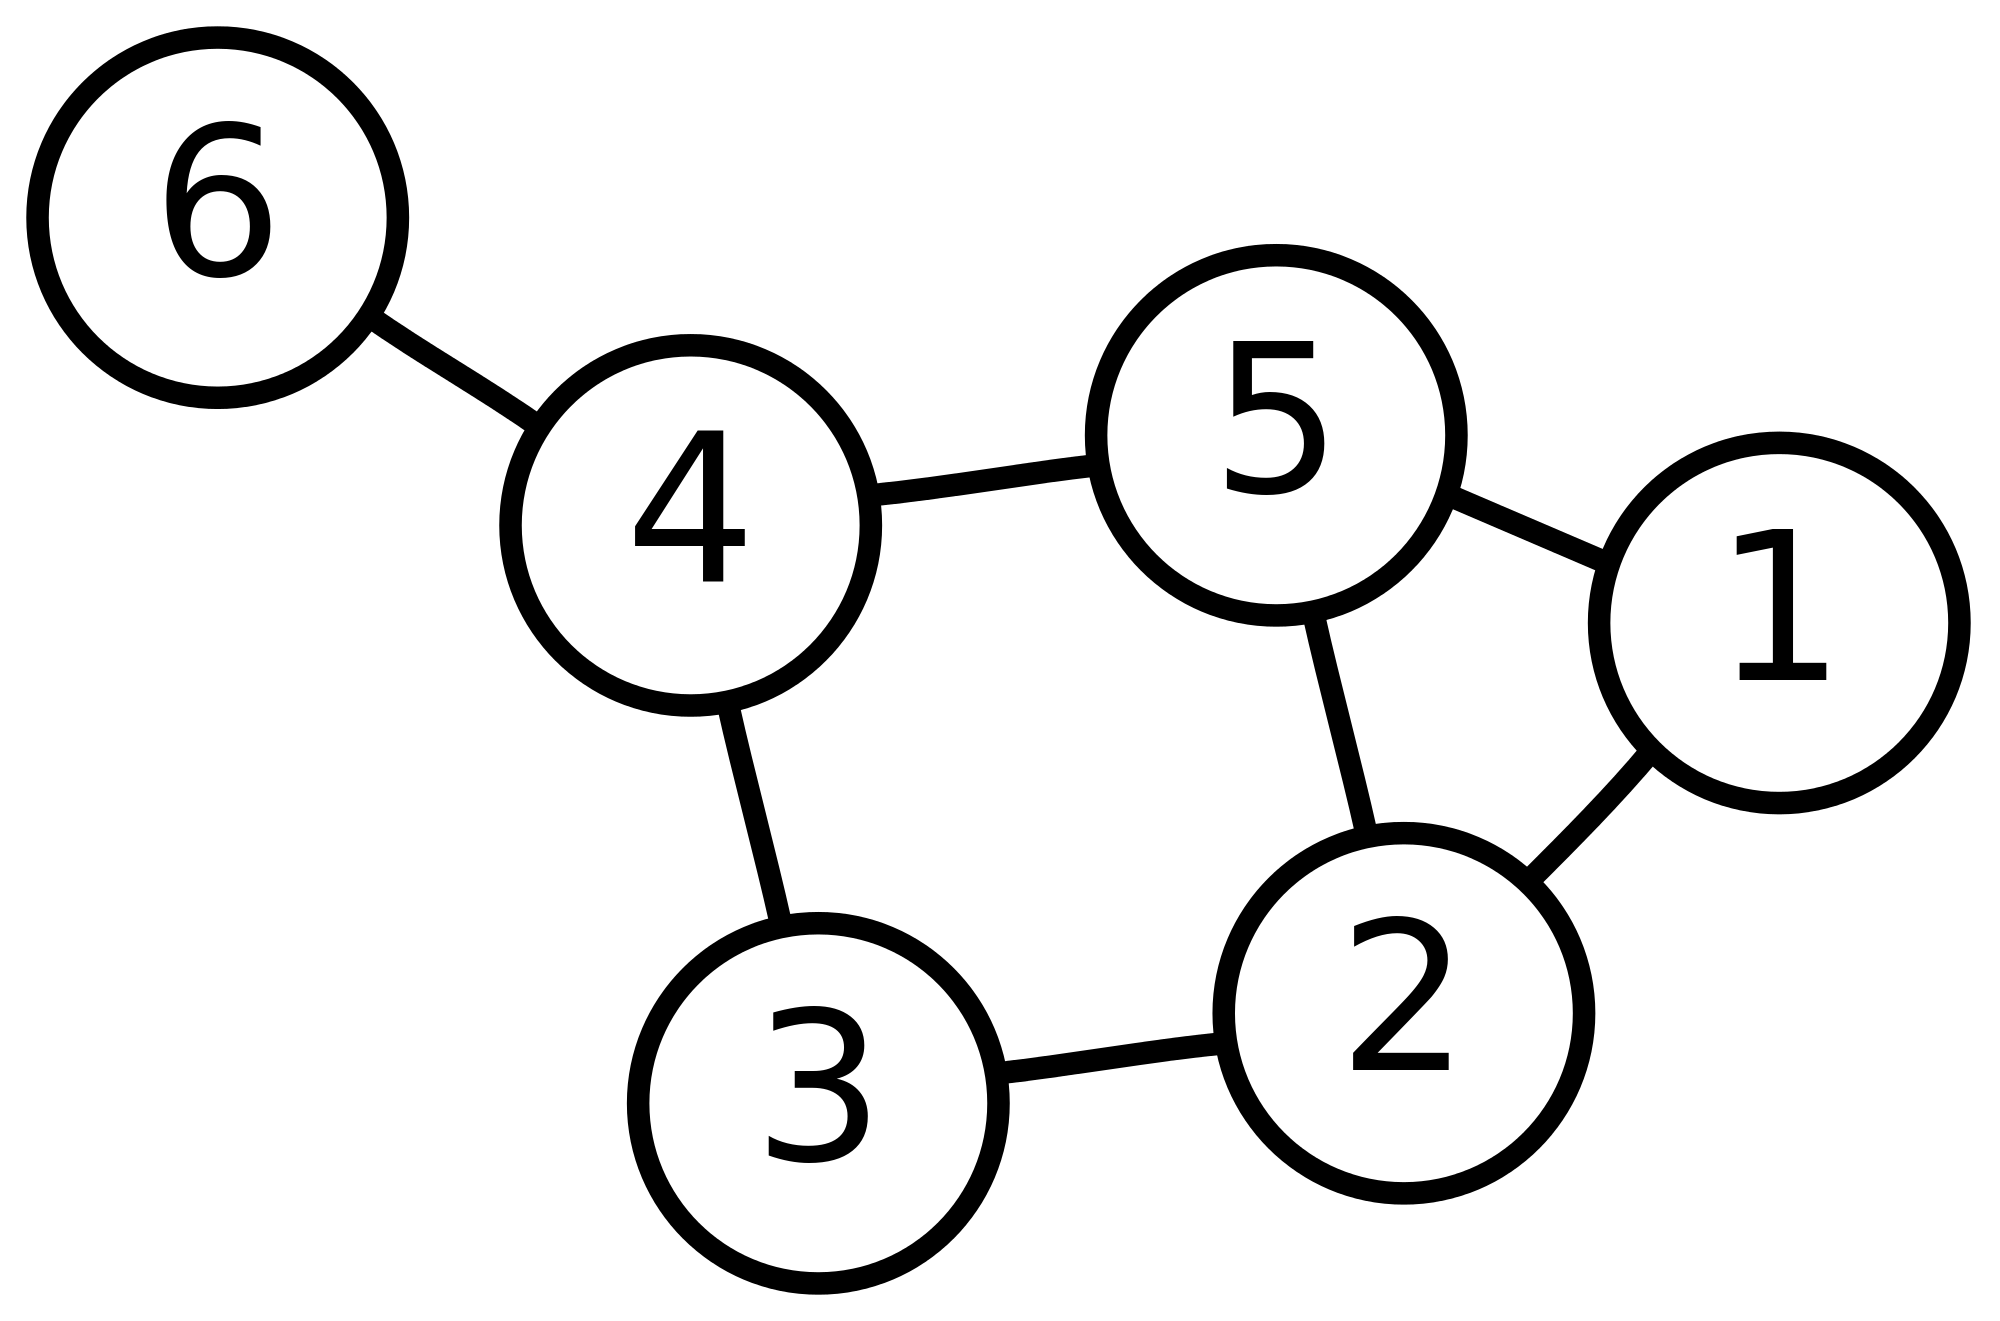
\includegraphics[scale=0.07]{./figures/graph_dfs_bfs.png}
	\end{columns}
	
	\begin{flushright} 
	Time complexity: \textbf{O(V+E)}
	\end{flushright}
\end{frame}

%%%%%%%%%%%%%%%%%%%%%%%%%%%%%%
\begin{frame}[plain]
\frametitle{}
\begin{center}
\Huge{\color{blue}{Q \& A}} \\
\vspace{5mm}
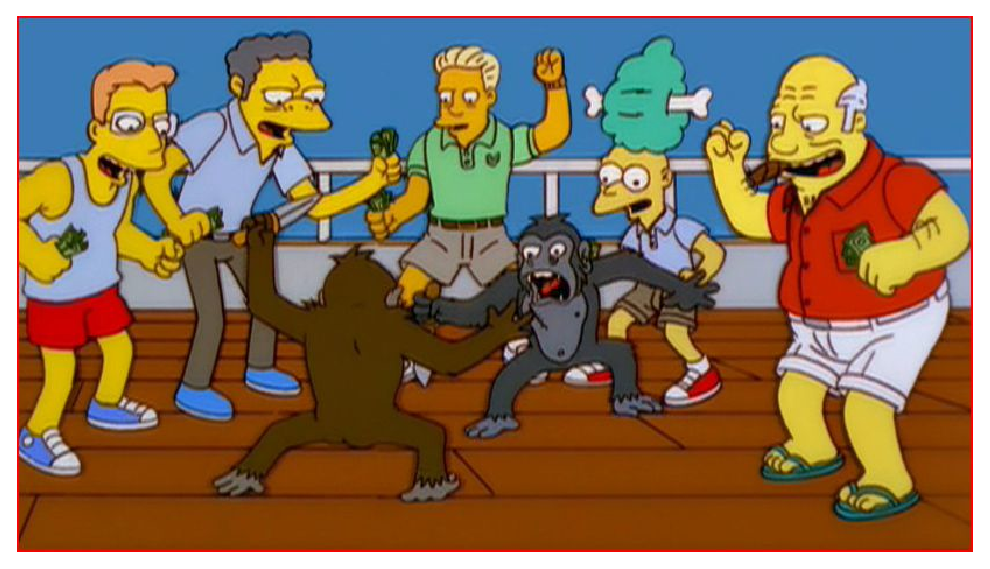
\includegraphics[scale=0.4]{./figures/monkey_fight.eps}
\end{center}
\end{frame}

%%%%%%%%%%%%%%%%%%%%%%%%%%%%%%%%
\begin{frame}[plain]
	\textbf{References}
	\begin{itemize}
		\item \href{https://sites.google.com/site/stevenhalim/}{Competitive Programming site}
		\item \href{https://github.com/davidjacobo/algorists/}{Algorists' repository}
	\end{itemize}
\end{frame}
\end{document}
